\chapter{Cycles et composantes connexes}

\section{Problèmes}

\begin{problem}
Soit $G = (S,\, A)$ et $u,\, v \in S$.\newline
Répondre $VRAI$ si il existe un chemin de $u$ à $v$ dans $G$, $FAUX$ sinon.
\label{problem1}
\end{problem}

\begin{problem}
Soit $G = (S,\, A)$ et $u,\, v \in S$.\newline
Est-ce qu'ajouter $(u,\, v)$ à $A$ crée un nouveau cycle ?
\label{problem2}
\end{problem}

\begin{proposition} 
Problème \ref{problem1} $\Leftrightarrow$ Problème \ref{problem2}
\end{proposition}

Si il existe un chemin de $u$ à $v$ : $u = u_1, u_2, ... u_k = v$ (qui ne passe pas 2 fois par le même sommet) alors il existe un cycle si on ajoute $u,\, v$.

Dans l'autre sens, si ajouter $(u,\, v)$ crée un nouveau cycle, alors il existe un chemin. En effet, si le morceau cycle passe par $u, v_1, ... v_k, u$ alors $G$ contient le chemin $u, v_k, ..., v_1, v$.

\begin{definition}\index{Composante connexe}
Une composante connexe d'un graphe $G = (S,\, A)$ est un sous-ensemble de sommets $S^{\prime} \subseteq S$ maximal tel que $\forall u,\, v \in S^{\prime}$, il existe un chemin de $u$ à $v$ dans $G$.
\end{definition}

\begin{problem}
Soient  $G = (S,\, A)$ et $u, v \in S$, $u$ et $v$ sont-ils dans la même composante connexe ?
\label{problem3}
\end{problem}

\section{Application : Kruskal}


\begin{figure}[h]
	\centering
	\begin{tikzpicture}
		\GraphInit[vstyle=Normal]
		\tikzset{VertexStyle/.append  style={fill = node}}
		\tikzset{VertexStyle/.append  style={text = white}}
		\SetGraphUnit{1.5}
		\begin{scope}[rotate=90]
		\Vertices{circle}{A, B, D, C}
		\Edge[label=$1$](A)(B)
		\Edge[label=$2$](A)(C)
		\Edge[label=$4$](C)(B)
		\Edge[label=$4$](D)(B)
		\Edge[label=$1$](D)(C)
		\end{scope}
	\end{tikzpicture}
	%\caption{}
	\label{fig:chap2_graph1}
\end{figure}

Trier les arêtes : $(A, B) (C, D) (A, C) (B, C) (B, D)$

Ajouter dans l'ordre sans créer de cycle :

\begin{enumerate}

\item Ajouter $(A, B)$, 3 composantes connexes.

\begin{figure}[h]
	\centering
	\begin{tikzpicture}
		\GraphInit[vstyle=Normal]
		\tikzset{VertexStyle/.append  style={fill = node}}
		\tikzset{VertexStyle/.append  style={text = white}}
		\SetGraphUnit{1.5}
		\begin{scope}[rotate=90]
		\Vertices{circle}{A, B, D, C}
		\Edge(A)(B)
		\end{scope}
	\end{tikzpicture}
\end{figure}

\item Ajouter $(C, D)$, 2 composantes connexes.

\begin{figure}[h]
	\centering
	\begin{tikzpicture}
		\GraphInit[vstyle=Normal]
		\tikzset{VertexStyle/.append  style={fill = node}}
		\tikzset{VertexStyle/.append  style={text = white}}
		\SetGraphUnit{1.5}
		\begin{scope}[rotate=90]
		\Vertices{circle}{A, B, D, C}
		\Edge(A)(B)
		\Edge(C)(D)
		\end{scope}
	\end{tikzpicture}
\end{figure}

\item Ajouter $(A, C)$ ? Ok, $A$ et $C$ ne sont pas dans la même composante connexe.

\begin{figure}[h]
	\centering
	\begin{tikzpicture}
		\GraphInit[vstyle=Normal]
		\tikzset{VertexStyle/.append  style={fill = node}}
		\tikzset{VertexStyle/.append  style={text = white}}
		\SetGraphUnit{1.5}
		\begin{scope}[rotate=90]
		\Vertices{circle}{A, B, D, C}
		\Edge(A)(B)
		\Edge(C)(D)
		\Edge(A)(C)
		\end{scope}
	\end{tikzpicture}
\end{figure}

\item Ajouter $(B, C)$. Non.

\end{enumerate}

%\newline
Objectif : trouver un algorithme performant pour résoudre le problème \ref{problem1}.
